\chapter{Machine Learning on Vertical-Partitioned Dataset}
Vertical partitioning involves splitting a dataset based on features, where each data holder possesses a subset of the features for the same set of individuals. This differs from horizontal partitioning, where different entities hold data for different individuals. The goal is to enable collaborative learning without compromising the privacy of the individuals whose data is being used.\\
For example, consider two hospitals aiming to improve diagnostic models by pooling their patient data. Each hospital has different pieces of patient information (e.g., one has genetic data while the other has imaging data). Vertical partitioning allows these hospitals to build a comprehensive model using their combined data without sharing their raw datasets.

\textbf{Private Set Intersection:}
Private Set Intersection (PSI) is a cryptographic technique that enables two parties to compute the intersection of their datasets without revealing any non-intersecting elements. This ensures that only the common elements are identified and used for further analysis.\\
PSI is crucial in vertical partitioning because it allows different entities to match records corresponding to the same individual without sharing sensitive information. For instance, if a pharmaceutical company wants to collaborate with a hospital to identify patients who have received a particular treatment and also have specific genetic markers, PSI can be employed. This method ensures that neither party learns more than necessary about the other's dataset.\\
There are several variations of PSI, each offering different trade-offs between computational efficiency and security. Basic PSI protocols often rely on cryptographic primitives such as hashing, oblivious transfer, and homomorphic encryption. Advanced PSI protocols improve efficiency and scalability, making them suitable for large datasets often encountered in real-world applications.

\textbf{Split Neural Network:}
Split Neural Networks (SplitNN) provide another approach to vertical partitioning by distributing the training of a neural network across multiple parties. In SplitNN, each party trains a portion of the network up to a certain layer, then passes the intermediate results (activations) to the next party. This process continues until the final output layer is reached.\\
The key advantage of SplitNN is that it keeps the raw data within each party's domain, only sharing the intermediate activations. This greatly enhances data privacy while still allowing for collaborative model training. For example, in a healthcare scenario, one hospital could train the initial layers of a neural network on imaging data, pass the intermediate activations to another hospital, which then continues training on genetic data.\\
SplitNN also offers the flexibility to handle different types of data and model architectures, making it suitable for various machine learning tasks. Additionally, it supports both supervised and unsupervised learning, further broadening its applicability.


\section{PSI Protocol and implementation}
\label{sec:PSI_protocol_implementation}
One widely used application of MPC is \textbf{Private Set Intersection} (\textbf{PSI}), which allows to compute the common elements between datasets' parties (for simplicity, we will focus on two parties).
Given a party $P_i$ with a dataset $D^i$, $i=1,2$, we want to compute $D^1 (j) \cap D^2 (j)$ being $D^i(j)$ the j-th column (set) from the i-th party's dataset. For example, if $D$ consist in a single list of phone numbers, $D^1 \cap D^2$ would be the common phone contacts between party 1 and party 2. Another example could be that the datasets $D^1$ and $D^2$ have the fields:\\

\begin{minipage}{0.4\textwidth}
\begin{itemize}
    \item $D^1(1) \coloneqq$ National Identity Number
    \item $D^1(2) \coloneqq$ Name
    \item $D^1(3) \coloneqq$ Surname
    \item $D^1(4) \coloneqq$ Annual Salary (\$)
\end{itemize}
\end{minipage}
\begin{minipage}{0.4\textwidth}
\begin{itemize}
\item $D^2(1) \coloneqq$ National Identity Number
\item $D^2(2) \coloneqq$ Age
\item $D^2(3) \coloneqq$ Genre
\end{itemize}
\end{minipage}

\vspace*{1 em}

If we would like to know the mean annual salary by genre, first we would need to \textit{merge} both datasets, mapping the National Identity Number.
With PSI, we could compute $D^1(1) \cap D^2(1)$, this  gives us the NIN of the people with complete data, i.e. the people whose personal data are in both datasets, so it is known both the annual salary and the genre.
With that intersection, we could get two subsets from $D^1$ and $D^2$ and then use another MPC protocol (in this case, we are interested in the operation \textit{GroupBy}).\\

As an informal introduction of the problem, we will develop the protocol studied in \cite{agrawal}. We define two sets: $V_A = \{v_1,\cdots, v_n\}$ and $V_B = \{v'_1,\cdots, v'_m\}$, $n,m\in\mathbb{N}$ which belong to node Alice and Bob resp.
For this protocol, it is needed a commutative encryption $\mathcal{F}$: a computable, in polynomial time, function $f \colon Key(\mathcal{F}) \times Dom(\mathcal{F}) \to Dom(\mathcal{F})$, defined on a finite domain, that satisfies the properties:

\begin{itemize}
    \item Commutativity: $\forall e, e' \in Key(\mathcal{F})$, $f_e \circ f_{e'} = f_{e'} \circ f_e$
    \item $f_e \colon Dom(\mathcal{F}) \to Dom(\mathcal{F})$ is a bijection $\forall e \in Key(\mathcal{F})$
    \item $f_e^{-1}$ is also computable in polynomial time given $e$.
    \item Given a value $x$ and its encryption $f_e (x)$, for a new value $y$ we cannot distinguish between $f_e(y)$ and a random value $z$ in polynomial time.
\end{itemize}

Let $Dom(F)$ be all quadratic residues modulo $p$, where $p$ is a "safe" prime number (both $p$ and $q = \frac{p-1}{2}$ are primes). Let $Key(\mathcal{F})$ be $\{1,2,...,q-1\}$. Then, the power function $f_e(x) \equiv x^e mod(p)$ is a commutative encryption.\\
In order to map the elements from $X$ and $Y$ (which are assumed to be set of unique elements, such as NIN) into $Dom(\mathcal{F})$, we need a hash function $h \colon V \to Dom(\mathcal{F})$, $V_A \cup V_B \subset V$, that can be considered computed by a random oracle: for each $v \in V$, an independent random $x \in_r Dom(\mathcal{F})$\footnote{$\in_r$ means: chosen uniformly at random from} is chosen for $x = h(v)$.
In order to avoid a collision, $|Dom(\mathcal{F}) >> |X \cup Y|$. Let $N = |Dom(\mathcal{F})|$, in the random oracle model the probability that $n$ hash values have at least one collision is:

\begin{equation*}
    P(hash \hspace*{0.3 em} collision) = 1 - \prod_{i=1}^{n-1} \frac{N-i}{N} \approx 1 - \exp \bigl( \frac{-n (n-1)}{2N} \bigr)
\end{equation*}

The intersection protocol described in \cite{agrawal} is:

\begin{algorithm}
\caption{Private Set Intersection Protocol}
\label{alg:PSI}
\begin{algorithmic}[1]
    \State Both Alice and Bob apply the hash function $h$ to their sets: $X_A = h(V_A)$ and $X_B = h(V_B)$. Each party randomly chooses a secret key: $e_A \in \text{Key}_F$ for Alice and $e_B \in \text{Key}_F$ for Bob.
    \State Both parties encrypt their hashed sets: $Y_A = f_{e_A}(X_A) = f_{e_A}(h(V_A))$ and $Y_B = f_{e_B}(X_B) = f_{e_B}(h(V_B))$.
    \State Bob sends to Alice his encrypted set $Y_B = f_{e_B}(h(V_B))$, reordered lexicographically.
    \State Alice sends to Bob her set $Y_A = f_{e_A}(h(V_A))$, reordered lexicographically.
    \State Alice encrypts each $y \in Y_B$ with her key $e_A$ and sends back to Bob pairs $\langle y, f_{e_A}(y) \rangle = \langle f_{e_B}(h(v)), f_{e_A}(f_{e_B}(h(v))) \rangle$.
    \State Bob encrypts each $y \in Y_A$ with $e_B$, obtaining $Z_A = f_{e_B}(f_{e_A}(h(V_A)))$. Also, from pairs $\langle f_{e_B}(h(v)), f_{e_A}(f_{e_B}(h(v))) \rangle$ obtained in Step 4(b) for $v \in V_B$, he creates pairs $\langle v, f_{e_A}(f_{e_B}(h(v))) \rangle$ by replacing $f_{e_B}(h(v))$ with the corresponding $v$.
    \State Bob selects all $v \in V_B$ for which $f_{e_A}(f_{e_B}(h(v))) \in Z_A$; these values form the set $V_A \cap V_B$.
\end{algorithmic}
\end{algorithm}

Note that Algorithm \ref{alg:PSI} can be modified so all the transmission operations are symmetrical, therefore both Alice and Bob know $V_A \cap V_B$. A toy implementation\footnote{Source code in \url{https://github.com/JSempereH/PSI_toy}} has been done in Python using gRPC, although this is a very basic implementation and shouldn't be considered for commercial use, since it has no guaranties of security nor privacy.

For learning purposes, let's suppose Alice has a dasatet with the following NINs: $12345678A$, $87654321B$, $54321678C$, $67891234D$, and Bob has a dataset with the following NINs: $67891234D$, $22222222Y$, $54321678C$, $11111111X$. Using a non-cryptographic hash function\footnote{We don't need a secure hash function, since only serves to map strings to $Dom(\mathcal{F})$. In the implementation, we use SHA1 \cite{sahu2017}} we perform step 1 from Algorithm \ref{alg:PSI}:

\begin{itemize}
    \item $X_A = [ 6801962795022291115, \hspace*{.2 em} 14914775733042932484, \hspace*{.2 em}  6031741069150041195, \hspace*{.2 em} 7775431530089967261] $
    \item $X_B = [ 7775431530089967261, \hspace*{.2 em}  15704629945399610882, \hspace*{.2 em}   6031741069150041195, \hspace*{.2 em} 8717288097697391268]$
\end{itemize}

Using $p=9223372036854771239$ and $q=4611686018427385619$, Alice's secret key $e_A = 2671390701970302872$ and Bob's secret key $e_B = 325637035052474817$, we perform step 2 encrypting $x^{e} \hspace*{0.2 em} mod(p)$ for $x \in X_A, X_B$ and $e \in e_A, e_B$:

\begin{itemize}
    \item $Y_A = [4037654302475096183, \hspace*{.2 em} 7215131381927850152, \hspace*{.2 em}  7524770399191986516, \hspace*{.2 em} 4530009952158919715]$
    \item $Y_B = [ 709144700394714309, \hspace*{.2 em} 1186382732300108902, \hspace*{.2 em}  683568481448076414, \hspace*{.2 em} 3441729271243177027]$
\end{itemize}

Both parties send its sets reordered (denoted by $\hat{Y}$), Bob receives Alice's ordered set and after encrypting, Bob sends back to Alice the set:

\begin{itemize}
    \item $f_{e_B}(\hat{Y}_A) = [5211193962823641457, \hspace*{.2 em} \mathbf{7666888661095677275}, \hspace*{.2 em} 4407230382765344063, \hspace*{.2 em} \mathbf{3478216981347847458}]$
\end{itemize}

Symmetrically, Alice receives Bob's ordered set and after encrypting, Alice sends back to Bob the set:
\begin{itemize}
    \item $f_{e_A}(\hat{Y}_B) = [\mathbf{3478216981347847458},\hspace*{.2 em} \mathbf{7666888661095677275}, \hspace*{.2 em} 8512757503240690236, \hspace*{.2 em} 6052532624285366477]$
\end{itemize}

Since we are using a commutative encryption scheme, $f_{e_A} \circ f_{e_B} = f_{e_B} \circ f_{e_A}$, each party can compare the received set w.r.t the one encrypted and, using the same indexes obtained by ordering in step 2, both parties would get that the common NINs are $67891234D$ and $54321678C$. This exact example can be executed in the script \textbf{PSI.py} in the source code.

\section{Split Neural Network}

It can be the case where different parties have vertical partitioned data where the label of interesting (in a classification task) is only present in one of them. In this case, the features may be in one party and the labels in the other. We could use PSI (see Section \ref{sec:PSI_protocol_implementation}) in order to get the common subset and align the datasets.
However, we can't use a distributed Machine Learning like the one explained in Section \ref{ch:Federated_Learning}, since the datasets are different across parties, therefore there isn't a common model architecture and we can't simply average the gradients. What we could do is \textit{split} a neural network, with its first layers being adequate for the first party and last layers being appropriate for the second one.\\
Let's suppose Alice has the features $\boldsymbol{x}$ and Bob the labels $y$, and the datasets are already aligned. Following the notation in Section \ref{sec:Multilayer_Perceptron}, we could summarize the steps as:


\begin{algorithm}
\caption{Example of SplitNN for 2 parties}
\label{alg:SplitNN}
\begin{algorithmic}[1]
    \State Alice initializes the weights of its split $F_A = \{\boldsymbol{z}_0,...,\boldsymbol{z}_n\}$
    \State Bob initializes the weights of its split $F_B = \{\boldsymbol{z}_{n+1},...,\boldsymbol{z}_N\}$
    \State \textbf{While} Alice has new data to train on and $epoch < MAX\_EPOCHS$  \textbf{do}
    \State \hspace*{1 em} Alice uses standard forward propagation on data and sends $\boldsymbol{z}_n = \psi(\boldsymbol{W}_n \boldsymbol{z}_{l-1} + \boldsymbol{b}_l)$ to Bob.
    \State \hspace*{1 em} Bob uses the received $\boldsymbol{z}_n$ as an input to its split $F_B$ and get the output $\boldsymbol{z}_N$.
    \State \hspace*{1 em} Bob computes the gradients of $F_B$ using Backpropagation and updates its weights.
    \State \hspace*{1 em} Bob sends the gradient of $\boldsymbol{z}_n$ to Alice.
    \State \hspace*{1 em} Alice backpropagates gradients received updating the weights of $F_A$.
\end{algorithmic}
\end{algorithm}

Unlike FL, the computation and communication cost is very low in SplitNN. Moreover, aside from the transmission of gradients, the neural network architecture would be identical to that of a centralized model, thus achieving similar performance. For more information on this type of framework and a generalization for $N$ parties see \cite{gupta2018}.
A basic implementation can be found in the source code of this work.\footnote{https://github.com/JSempereH/TFM/tree/main/src/}. For Alice, a multilayer perceptron with a first layer of $784$ units, a hidden layer of $128$ and another one of $640$, all fully connected layers with ReLU activation functions (see Section \ref{sec:Multilayer_Perceptron} for more information). For Bob, a layer of $640$ units with ReLU and an output layer of $10$ units with LogSoftMax activation function (for a classification task). It has been trained with MNIST dataset (see \cite{deng2012} for more information about this dataset) during 10 epochs following Algorithm \ref{alg:SplitNN}.
\begin{figure}[H]
  \centering
  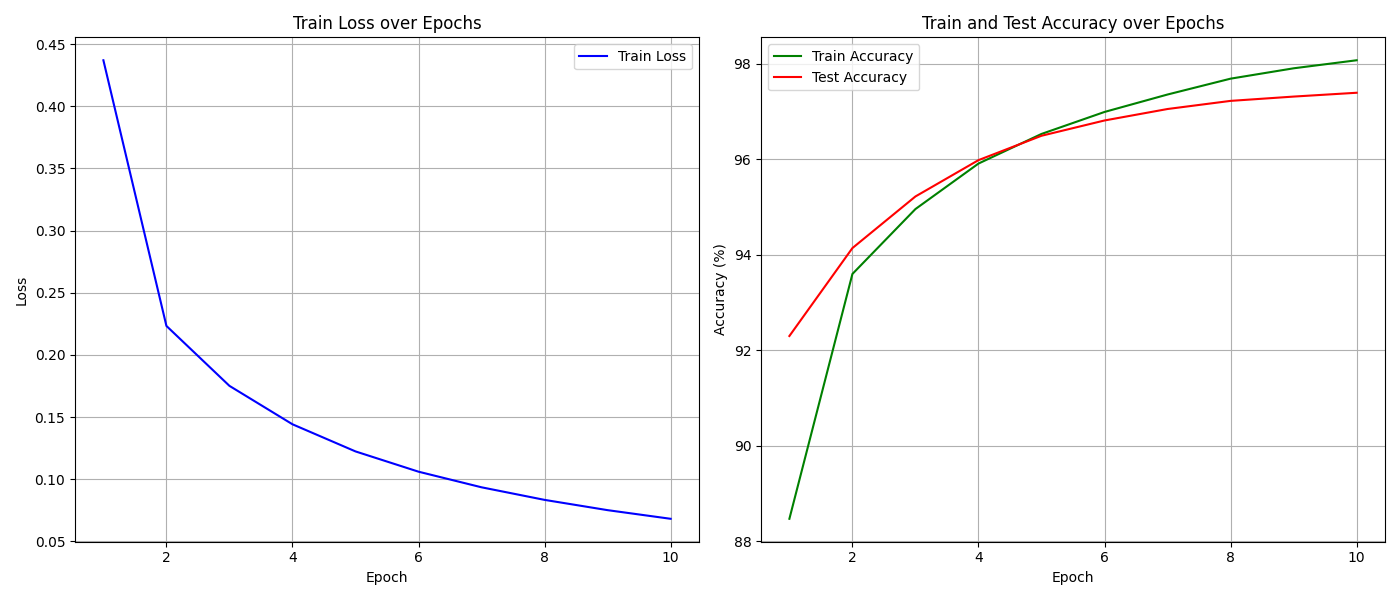
\includegraphics[width=0.6\textwidth]{figures/3-Vertical_Machine_Learning/MNIST_metrics_SplitNN.png}
  \caption{Example of SplitNN using MNIST dataset. The training performs the same as a centralized model.}
  \label{fig:MNIST_SplitNN_Metrics}
\end{figure}

Of course, there are many more algorithms for training models on vertically partitioned data.
A fairly comprehensive list of VFL algorithms can be found in \cite{yang2023}. Most techniques require the use of homomorphic encryption or MPC. These technologies are beyond the scope of this work, but I recommend checking \cite{gentry}, \cite{escudero2022} and \cite{evans} for an introduction.
